\section{Expert Reviews / Inspections}

Per valutare la qualità complessiva dell’esperienza utente e la coerenza progettuale del sistema, è stata pianificata una revisione sistematica dell’interfaccia basata su una \textbf{valutazione euristica} secondo i principi di Nielsen \cite{nielsen1995}.  
L’attività ha avuto l’obiettivo di identificare punti di forza, criticità e incoerenze nel design, analizzando in due fasi distinte il \textit{prototipo realizzato in Figma} e successivamente la \textit{versione web implementata}.  

La revisione del prototipo Figma ha rappresentato un passaggio fondamentale prima dello sviluppo effettivo: ha consentito di riflettere in modo critico sulle scelte di interfaccia, di validare le principali logiche di navigazione e di anticipare eventuali problemi di usabilità.  
A differenza della versione web, il prototipo non consente un’interazione reale, ma offre comunque una base solida per verificare la chiarezza dei flussi e la coerenza visiva complessiva.

\subsection*{Obiettivi della Review}

Gli obiettivi principali dell’attività di \textit{Expert Review} sono stati:
\begin{itemize}
    \item Valutare la \textbf{usabilità} dei flussi principali del sistema, verificando la chiarezza dei percorsi e delle azioni disponibili.
    \item Analizzare la \textbf{coerenza visiva} rispetto alle linee guida di design definite nel brand e nel prototipo.
    \item Individuare problemi di \textbf{chiarezza, navigabilità e feedback} che possano compromettere l’esperienza d’uso.
    \item Identificare eventuali mancanze o ridondanze, con l’obiettivo di \textbf{migliorare la struttura informativa e la consistenza visiva}.
    \item Definire raccomandazioni per le fasi successive di sviluppo, in vista della revisione della \textbf{versione web funzionante}.
\end{itemize}

\subsection*{Motivazione della Checklist Scelta}

Per garantire una valutazione sistematica, replicabile e comparabile tra diverse aree dell’interfaccia, è stata utilizzata una \textbf{checklist di usabilità} costruita sui dieci principi di Nielsen.  
Questo approccio è stato scelto perché:
\begin{itemize}
    \item consente una \textbf{autovalutazione strutturata} anche in assenza di utenti reali o revisori esterni;
    \item può essere applicato sia a \textbf{prototipi statici} (come quelli sviluppati in Figma) sia a \textbf{interfacce interattive} e funzionanti;
    \item copre in modo ampio le dimensioni fondamentali dell’usabilità: visibilità dello stato del sistema, coerenza, prevenzione degli errori, efficienza, chiarezza e supporto all’utente.
\end{itemize}

\subsection*{Struttura della Checklist Euristica}

La checklist adottata si basa sui dieci principi classici di Nielsen, riformulati in forma di domande operative per adattarli al contesto del progetto.  
Ogni criterio è stato utilizzato come base per analizzare il prototipo Figma e successivamente la versione web.

\begin{table}[H]
\centering
\begin{tabular}{p{0.7cm} p{4cm} p{8cm}}
\hline
\textbf{\#} & \textbf{Criterio} & \textbf{Domanda di verifica} \\
\hline
1 & Visibilità dello stato del sistema & L’utente riceve sempre un feedback visivo o testuale dopo un’azione (salvataggio, invio, errore)? \\
2 & Corrispondenza tra sistema e mondo reale & Terminologia, icone e messaggi sono coerenti con il linguaggio del dominio immobiliare? \\
3 & Controllo e libertà dell’utente & È possibile annullare o correggere facilmente un’azione? \\
4 & Coerenza e standard & Colori, stili e componenti rispettano il design definito nel brand e nel prototipo? \\
5 & Prevenzione e gestione degli errori & I form prevengono gli errori tramite validazioni e messaggi chiari? \\
6 & Efficienza e flessibilità d’uso & Le operazioni più frequenti possono essere eseguite rapidamente, anche da dispositivi mobili? \\
7 & Chiarezza del contenuto & Testi e etichette sono comprensibili e privi di ambiguità? \\
8 & Supporto al riconoscimento & Le opzioni principali sono visibili e non richiedono memoria a breve termine all’utente? \\
9 & Feedback e conferme & Sono presenti messaggi di conferma dopo azioni critiche (pubblicazione, eliminazione, invio)? \\
10 & Aiuto e documentazione & È disponibile un supporto o una guida per l’utente in caso di difficoltà? \\
\hline
\end{tabular}
\caption{Checklist di valutazione euristica basata sui principi di Nielsen.}
\end{table}

\bigskip

La sezione seguente presenta nel dettaglio l’applicazione di questa checklist al \textbf{prototipo Figma}, con un’analisi critica dei dieci criteri e una successiva autovalutazione sintetica dei risultati ottenuti.

\subsection{Expert Review sul Prototipo Figma}

L’attività di revisione euristica è stata condotta sul prototipo sviluppato in \textit{Figma} prima della realizzazione della versione web.  
L’obiettivo è stato valutare il livello di usabilità e coerenza delle principali interfacce progettate, verificando la presenza di feedback, la chiarezza dei flussi e la consistenza grafica secondo i dieci principi di Nielsen.  

\subsubsection*{1. Visibilità dello stato del sistema}  
Nel prototipo sono stati previsti diversi meccanismi di feedback.  
Nei flussi \textit{Fai controproposta} e \textit{Registra dipendente} sono stati inseriti \textbf{indicatori di caricamento} per mostrare lo stato del sistema durante le operazioni.  
In tutti i form è presente un \textbf{sistema di validazione immediata}: i campi non validi vengono evidenziati in rosso e, nel caso della \textit{creazione di un annuncio}, il processo è suddiviso in step.  
Quando uno step contiene errori, il suo indicatore cambia colore e un box iniziale riepiloga i campi non validi.  
Tutti i flussi analizzati includono un \textbf{doppio messaggio di conferma} prima dell’esecuzione definitiva, ad eccezione della creazione di un annuncio.  
Nel complesso, il prototipo offre una buona visibilità dello stato del sistema, con l’unica criticità relativa all’assenza di conferma dopo la pubblicazione.

\subsubsection*{2. Corrispondenza tra sistema e mondo reale}  
Il linguaggio utilizzato è \textbf{semplice e diretto}, adatto agli utenti finali.  
Le sezioni con terminologia più specifica (legate alle agenzie immobiliari) risultano coerenti con il dominio e adatte a un pubblico professionale.  
Sono state impiegate \textbf{icone standard e universalmente riconoscibili}, affiancate da \textbf{tooltip descrittivi} che ne chiariscono il significato.  
L’unico aspetto ancora da migliorare riguarda la \textbf{scelta delle icone nello stepper} di creazione annuncio, dove sarebbe utile uno studio mirato per rendere più intuitivi i passaggi.

\subsubsection*{3. Controllo e libertà dell’utente}  
Il prototipo garantisce buone possibilità di annullamento e controllo.  
Tutti i popup includono una \textbf{“X” per chiudere o annullare}, e i messaggi di conferma prevedono esplicitamente un pulsante \textit{Annulla}.  
Le azioni potenzialmente distruttive, come la \textbf{disattivazione delle notifiche}, richiedono conferma; viceversa, l’attivazione non la richiede poiché non comporta rischi di perdita di dati.  
La progettazione su questo punto è stata ritenuta soddisfacente e coerente con le aspettative di usabilità.

\subsubsection*{4. Coerenza e standard}  
Il design mantiene nel complesso una \textbf{coerenza visiva} nei colori e nello stile dei pulsanti, in linea con il concept minimalista del progetto.  
Tuttavia, si è rilevata una \textbf{mancanza di uniformità nei popup}: nei diversi casi d’uso sono stati utilizzati modelli leggermente differenti, frutto di sperimentazioni grafiche ancora non consolidate.  
In fase di sviluppo sarà necessario \textbf{uniformare componenti e modali}, garantendo una coerenza piena tra tutti i flussi.

\subsubsection*{5. Prevenzione e gestione degli errori}  
La prevenzione degli errori è uno degli aspetti più curati nel prototipo.  
I form mostrano in tempo reale i campi non validi e forniscono \textbf{indicazioni visive chiare (rosso)} insieme a messaggi testuali.  
La combinazione di validazione immediata e conferme d’azione riduce significativamente il rischio di errori da parte dell’utente.  
Questo punto risulta pienamente soddisfatto.

\subsubsection*{6. Efficienza e flessibilità d’uso}  
Essendo un prototipo statico, l’efficienza d’uso è valutabile solo in parte.  
L’interfaccia è stata progettata per un utilizzo anche da \textbf{dispositivi verticali}, ma la resa migliore si ottiene in \textbf{orientamento orizzontale (landscape)}.  
Non sono state ancora considerate \textbf{scorciatoie o funzionalità avanzate} per utenti esperti (es. salvataggio bozza, importazione di dati da file), che potrebbero rappresentare un’evoluzione futura del progetto.  
Si riconosce quindi questo come un punto da sviluppare ulteriormente.

\subsubsection*{7. Chiarezza del contenuto}  
I testi sono \textbf{brevi, diretti e privi di tecnicismi}, con un linguaggio coerente e immediato.  
Quando una sola etichetta non è sufficiente, è previsto l’uso di \textbf{tooltip esplicativi}.  
Questo approccio consente una buona comprensione del flusso anche senza documentazione aggiuntiva.

\subsubsection*{8. Supporto al riconoscimento}  
Le principali funzioni sono \textbf{raggiungibili in pochi clic}.  
La \textit{header bar} consente di passare rapidamente tra ricerca, storico annunci e notifiche; inoltre, il passaggio tra l’area cliente e quella agenzia è reso accessibile dal \textit{footer}.  
Un test di eye-tracking condotto su alcune schermate del prototipo ha confermato la \textbf{corretta collocazione visiva} degli elementi più rilevanti, validando l’efficacia della struttura.

\subsubsection*{9. Feedback e conferme}  
Le operazioni critiche, come eliminazione o modifica, utilizzano lo stesso colore principale del sito, il che può generare confusione con azioni neutre.  
Si suggerisce di differenziare \textbf{visivamente le azioni distruttive} (es. usando toni di rosso o arancione) e di inserire messaggi di conferma più evidenti per i processi più delicati.  
Nonostante ciò, il comportamento rimane accettabile per utenti esperti.

\subsubsection*{10. Aiuto e documentazione}  
Non è stato previsto un sistema di aiuto, documentazione o FAQ, poiché il prototipo nasce in un contesto accademico.  
Tuttavia, in una versione completa sarebbe opportuno introdurre:  
\begin{itemize}
    \item una \textbf{sezione FAQ} o assistenza per i problemi più comuni;  
    \item \textbf{overlay o onboarding guidato} per i nuovi utenti;  
    \item pulsanti contestuali “Come funziona” nelle pagine più complesse.  
\end{itemize}

\subsubsection*{Autovalutazione e sintesi}  
La tabella seguente riassume il livello di soddisfacimento delle euristiche sul prototipo Figma (0 = non soddisfatto, 1 = parzialmente soddisfatto, 2 = soddisfatto).

\begin{table}[h!]
\centering
\begin{tabular}{p{0.4cm} p{4cm} p{1.5cm} p{7cm}}
\hline
\textbf{\#} & \textbf{Criterio} & \textbf{Valutazione} & \textbf{Motivazione sintetica} \\ \hline
1 & Visibilità stato & 2 & Feedback e validazioni chiare, manca solo conferma finale in creazione annuncio \\
2 & Corrispondenza mondo reale & 2 & Linguaggio semplice e coerente, icone chiare \\
3 & Controllo e libertà & 2 & Annulla e conferme sempre presenti \\
4 & Coerenza e standard & 1 & Popup non uniformi tra i flussi \\
5 & Prevenzione errori & 2 & Validazione in tempo reale e segnalazioni visive \\
6 & Efficienza/flessibilità & 1 & Assenza di scorciatoie e ottimizzazione solo parziale per mobile \\
7 & Chiarezza del contenuto & 2 & Testi sintetici e coerenti \\
8 & Supporto al riconoscimento & 2 & Navigazione semplice e confermata da test visivi \\
9 & Feedback/Conferme & 1 & Colori azioni critiche da differenziare \\
10 & Aiuto/Documentazione & 0 & Non prevista sezione di supporto \\ \hline
\end{tabular}
\caption{Autovalutazione euristica del prototipo Figma secondo i principi di Nielsen.}
\end{table}

\subsubsection*{Conclusioni}  
Il prototipo Figma risulta \textbf{completo, coerente e ben strutturato}, con una gestione accurata dei form, validazioni efficaci e buona leggibilità generale.  
I principali margini di miglioramento riguardano la \textbf{coerenza visiva dei popup}, la \textbf{differenziazione dei feedback critici} e l’assenza di un \textbf{sistema di aiuto} o onboarding.  
Questi aspetti costituiranno la base per le iterazioni successive e per l’ottimizzazione della versione web finale.


\subsection{Iterazione sul Prototipo e Realizzazione della Versione Web}

Dopo la revisione euristica sul prototipo Figma, è stata avviata la realizzazione della versione web definitiva.
Il prototipo ha rappresentato il punto di partenza per la struttura e la logica dei flussi, ma in questa fase l’attenzione si è concentrata sull’uniformità visiva, sulla chiarezza dei feedback e sulla robustezza dei meccanismi di interazione.

\subsubsection*{Uniformità visiva tramite PrimeVue}
Per garantire coerenza grafica e semplicità di manutenzione, il frontend è stato sviluppato utilizzando il framework \textbf{PrimeVue}.
L’adozione di questa libreria ha permesso di centralizzare le configurazioni di stile e di utilizzare componenti visivi coerenti in tutto il sistema.
Grazie a questa scelta, i popup, i pulsanti, le form e le finestre modali seguono lo stesso schema cromatico e tipografico, assicurando uniformità tra tutti i flussi applicativi.
Le differenze grafiche riscontrate nel prototipo, in particolare nei modali di conferma e negli alert, sono state eliminate, ottenendo un’interfaccia più pulita e coerente.

Inoltre, negli step di creazione di un annuncio sono state introdotte icone rappresentative per ciascuna fase del processo (es. dettagli, immagini, pubblicazione).
Questo accorgimento ha migliorato la corrispondenza tra sistema e mondo reale, rendendo il flusso più intuitivo e riconoscibile anche a colpo d’occhio.
\textit{Le Figure~\ref{fig:popup-login} e~\ref{fig:popup-conferma} mostrano i popup uniformati, mentre le Figure~\ref{fig:stepper-prima} e~\ref{fig:stepper-dopo} illustrano rispettivamente la versione dello stepper prima e dopo l’introduzione delle icone.}

\begin{figure}[H]
\centering

\includegraphics[width=0.8\textwidth]{Immagini/Expert Reviews/Figma/StepperCreazioneAnnuncio.png}
\caption{Stepper originale senza icone descrittive.}
\label{fig:stepper-prima}
\end{figure}

\begin{figure}[H]
\centering

\includegraphics[width=0.8\textwidth]{Immagini/Expert Reviews/Sito/StepperCreazioneAnnuncio.png}
\caption{Stepper aggiornato con icone rappresentative per ogni fase.}
\label{fig:stepper-dopo}
\end{figure}


\vspace{4pt}
\textit{(Figura~\ref{fig:popup-login}) mostra il popup di login con stile uniforme, mentre la Figura~\ref{fig:popup-conferma} illustra un esempio di messaggio di conferma.}

\vspace{4pt}
\textit{Le Figure~\ref{fig:popup-login} e~\ref{fig:popup-conferma} mostrano rispettivamente il popup di login e quello di conferma, uniformati nello stile PrimeVue.}

\begin{figure}[H]
\centering
\begin{minipage}[t]{0.48\textwidth}
    \centering
    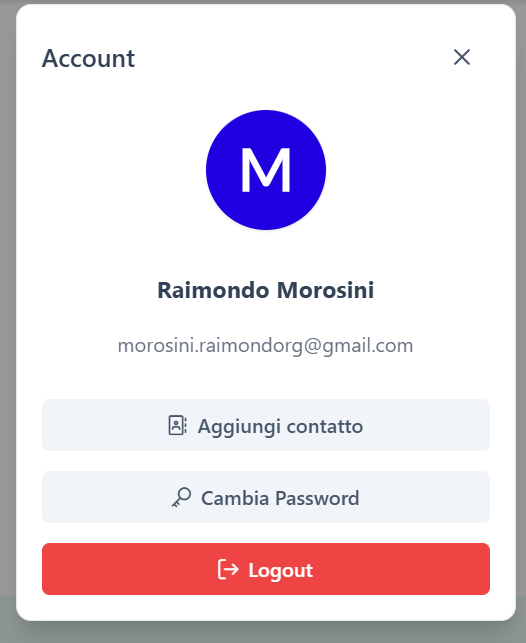
\includegraphics[width=\textwidth]{Immagini/Expert Reviews/Sito/PopupAccount.png}
    \caption{Popup di login con stile uniforme (PrimeVue).}
    \label{fig:popup-login}
\end{minipage}
\hfill
\begin{minipage}[t]{0.48\textwidth}
    \centering
    
\includegraphics[width=\textwidth]{Immagini/Expert Reviews/Sito/CreazioneAnnuncioConSuccesso.png}
    \caption{Esempio di popup di conferma operazione riuscita.}
    \label{fig:popup-conferma}
\end{minipage}
\end{figure}

\subsubsection*{Gestione degli errori e miglioramento del feedback}
Uno dei principali interventi rispetto al prototipo riguarda la gestione degli errori nel form di creazione di un annuncio.
Nel prototipo la validazione era presente ma meno visibile; nella versione web, per ogni step del processo, è stata introdotta una sezione evidenziata con sfondo rosso che riepiloga in modo chiaro tutti gli errori presenti.
In questo modo, l’utente può identificare immediatamente i campi errati senza doverli cercare manualmente, riducendo tempi e confusione.

\vspace{4pt}
\textit{(Figura~\ref{fig:errore-step}) mostra la nuova area di segnalazione errori all’interno dello step di creazione annuncio.}

\begin{figure}[H]
\centering
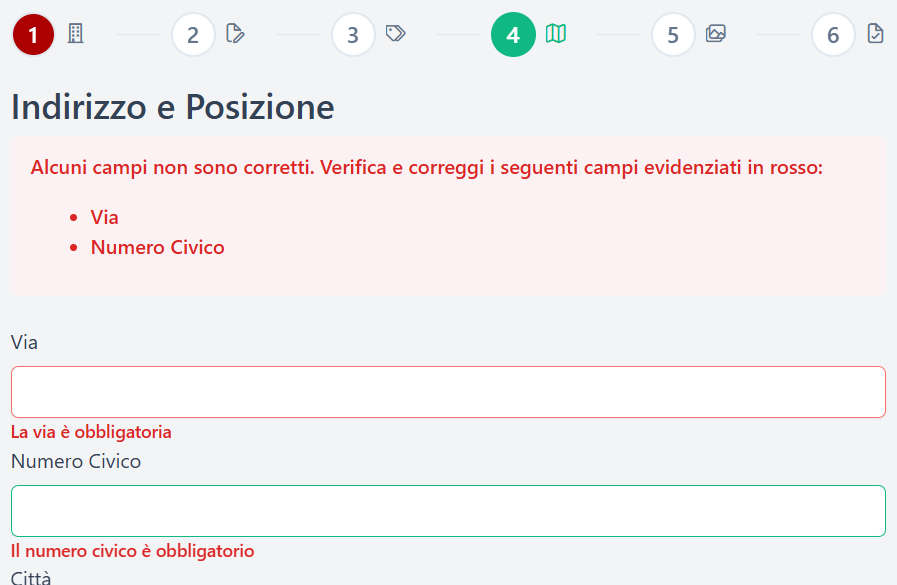
\includegraphics[width=0.8\textwidth]{Immagini/Expert Reviews/Sito/CreazioneAnnuncioConErrori.png}
\caption{Area di validazione con sfondo rosso nel form di creazione annuncio.}
\label{fig:errore-step}
\end{figure}

\subsubsection*{Conferme e messaggi di sistema}
Tutte le operazioni critiche o potenzialmente irreversibili (come eliminazione o pubblicazione) sono ora accompagnate da messaggi di conferma dedicati, garantendo un controllo maggiore da parte dell’utente.
Sono stati inoltre introdotti popup per notificare errori, conferme e caricamenti, tutti realizzati tramite componenti PrimeVue uniformi.

\vspace{4pt}
\textit{(Figura~\ref{fig:popup-errore}) e (Figura~\ref{fig:popup-success}) mostrano rispettivamente un messaggio di errore e una conferma di successo.}

\begin{figure}[H]
\centering
\begin{minipage}[t]{0.48\textwidth}
    \centering
    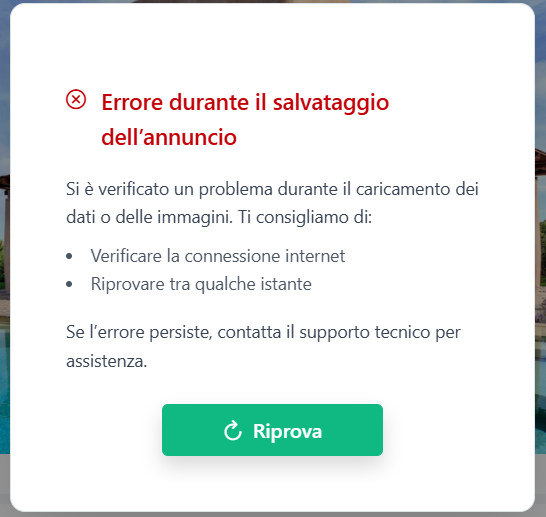
\includegraphics[width=\textwidth]{Immagini/Expert Reviews/Sito/CreazioneAnnuncioErrore.png}
    \caption{Esempio di popup di errore.}
    \label{fig:popup-errore}
\end{minipage}
\hfill
\begin{minipage}[t]{0.48\textwidth}
    \centering
    
\includegraphics[width=\textwidth]{Immagini/Expert Reviews/Sito/PopupRegistrazioneAccountGoogleGiaPresentepng.png}
    \caption{Esempio di stato di successo in un’operazione.}
    \label{fig:popup-success}
\end{minipage}
\end{figure}

\subsubsection*{Visibilità dello stato del sistema e animazioni}
Per migliorare la percezione di reattività, è stato aggiunto un indicatore di caricamento nelle fasi di attesa, come durante la ricerca di annunci o l’elaborazione di richieste.
A differenza del prototipo, dove si ipotizzava una progress bar, la versione web utilizza uno spinner circolare, più adatto per operazioni asincrone di durata variabile.
Lo spinner comunica all’utente che il sistema è attivo anche in assenza di un progresso misurabile, migliorando la trasparenza e riducendo l’ansia da attesa.

\vspace{4pt}
\textit{(Figura~\ref{fig:popup-loading}) mostra lo spinner di caricamento utilizzato nei popup.}

\begin{figure}[H]
\centering

\includegraphics[width=0.7\textwidth]{Immagini/Expert Reviews/Sito/CreazioneAnnuncioCaricamento.png}
\caption{Animazione di caricamento (spinner) durante operazioni asincrone.}
\label{fig:popup-loading}
\end{figure}

\subsubsection*{Sintesi dei miglioramenti principali}
La tabella seguente riassume le principali modifiche introdotte rispetto al prototipo Figma e i relativi benefici in termini di usabilità.

\begin{table}[H]
\centering
\setlength{\tabcolsep}{6pt}
\renewcommand{\arraystretch}{1.2}
\begin{tabular}{p{5cm} p{10cm}}
\hline
\textbf{Criticità nel prototipo} & \textbf{Soluzione implementata nella versione web} \\
\hline
Popup con stili differenti & Uniformati tramite componenti PrimeVue centralizzati \\
Assenza conferma creazione annuncio & Aggiunto popup di conferma prima della pubblicazione \\
Errori dispersi nel form & Introdotta sezione rossa riepilogativa per ogni step \\
Progress bar nei caricamenti & Sostituita con spinner per attese di durata variabile \\
Assenza icone negli step & Aggiunte icone descrittive per migliorare la comprensione visiva \\
Feedback visivo poco distinto & Differenziati colori per errori, successi e conferme \\
\hline
\end{tabular}
\caption{Sintesi dei miglioramenti principali introdotti nella versione web.}
\end{table}

\subsubsection*{Autovalutazione euristica della versione web}

È stata quindi condotta una nuova autovalutazione secondo i dieci principi di Nielsen, con l’obiettivo di verificare l’efficacia delle migliorie e individuare ulteriori aree di sviluppo.

\begin{table}[H]
\centering
\setlength{\tabcolsep}{6pt}
\renewcommand{\arraystretch}{1.2}
\begin{tabular}{p{0.4cm} p{4cm} p{1.5cm} p{7cm}}
\hline
\textbf{\#} & \textbf{Criterio} & \textbf{Valutazione} & \textbf{Motivazione sintetica} \\
\hline
1 & Visibilità stato & 2 & Spinner e messaggi di caricamento chiari in tutte le operazioni \\
2 & Corrispondenza mondo reale & 2 & Linguaggio coerente e icone aggiunte negli step migliorano la comprensione \\
3 & Controllo e libertà & 2 & Tutte le azioni critiche prevedono conferma e possibilità di annullamento \\
4 & Coerenza e standard & 2 & PrimeVue centralizza lo stile e uniforma i componenti grafici \\
5 & Prevenzione errori & 2 & Area rossa riepiloga errori per ogni step; validazione efficace \\
6 & Efficienza/flessibilità & 1 & Mancano shortcut, funzioni per utenti esperti e salvataggio bozza cross-device \\
7 & Chiarezza del contenuto & 2 & Testi sintetici e coerenti, layout leggibile anche su dispositivi diversi \\
8 & Supporto al riconoscimento & 2 & Navigazione intuitiva, icone e percorsi chiari tra le sezioni \\
9 & Feedback/Conferme & 2 & Popup coerenti per conferme, errori e caricamenti \\
10 & Aiuto/Documentazione & 0 & Assenti FAQ, onboarding e funzioni di accessibilità \\
\hline
\end{tabular}
\caption{Autovalutazione euristica della versione web secondo i principi di Nielsen.}
\end{table}

\subsubsection*{Analisi critica e prospettive di miglioramento}
La versione web rappresenta un’evoluzione matura e coerente del prototipo Figma, con un significativo miglioramento nella consistenza grafica, gestione degli errori e chiarezza dei feedback.
Tuttavia, l’analisi critica mette in evidenza alcune aree ancora aperte:
\begin{itemize}
\item \textbf{Accessibilità non implementata}: mancano funzioni per utenti con disabilità (navigazione da tastiera, supporto screen reader).
\item \textbf{Bozze non persistenti}: i dati sono salvati solo nel \textit{Pinia store} locale, quindi non recuperabili su dispositivi diversi.
\item \textbf{Mancanza di scorciatoie e funzioni avanzate} per utenti esperti.
\item \textbf{Assenza di FAQ o onboarding guidato} che agevolino la comprensione iniziale.
\item \textbf{Ottimizzazione mobile solo parziale}, soprattutto in visualizzazione verticale.
\end{itemize}
